%% Commands for TeXCount
%TC:macro \cite [option:text,text]
%TC:macro \citep [option:text,text]
%TC:macro \citet [option:text,text]
%TC:envir table 0 1
%TC:envir table* 0 1
%TC:envir tabular [ignore] word
%TC:envir displaymath 0 word
%TC:envir math 0 word
%TC:envir comment 0 0

\documentclass[sigconf]{acmart}


\usepackage{bbm}


%%
%% \BibTeX command to typeset BibTeX logo in the docs
\AtBeginDocument{%
  \providecommand\BibTeX{{%
    Bib\TeX}}}

\settopmatter{printacmref=false} % removes ACM reference format
\renewcommand\footnotetextcopyrightpermission[1]{} % removes footnote with conference info


\begin{document}

\title{SoccerCPD : Formation and Role Change-Point Detection in Soccer Matches Using Spatiotemporal Tracking Data}

\author{Adonis Jamal}
\email{adonis.jamal@student-cs.fr}
\affiliation{%
  \institution{CentraleSupélec}
  \city{Gif-sur-Yvette}
  \country{France}
}

\author{Fotios Kapotos}
\email{fotiskapotos@gmail.com}
\affiliation{%
  \institution{CentraleSupélec}
  \city{Gif-sur-Yvette}
  \country{France}
}

\begin{teaserfigure}
  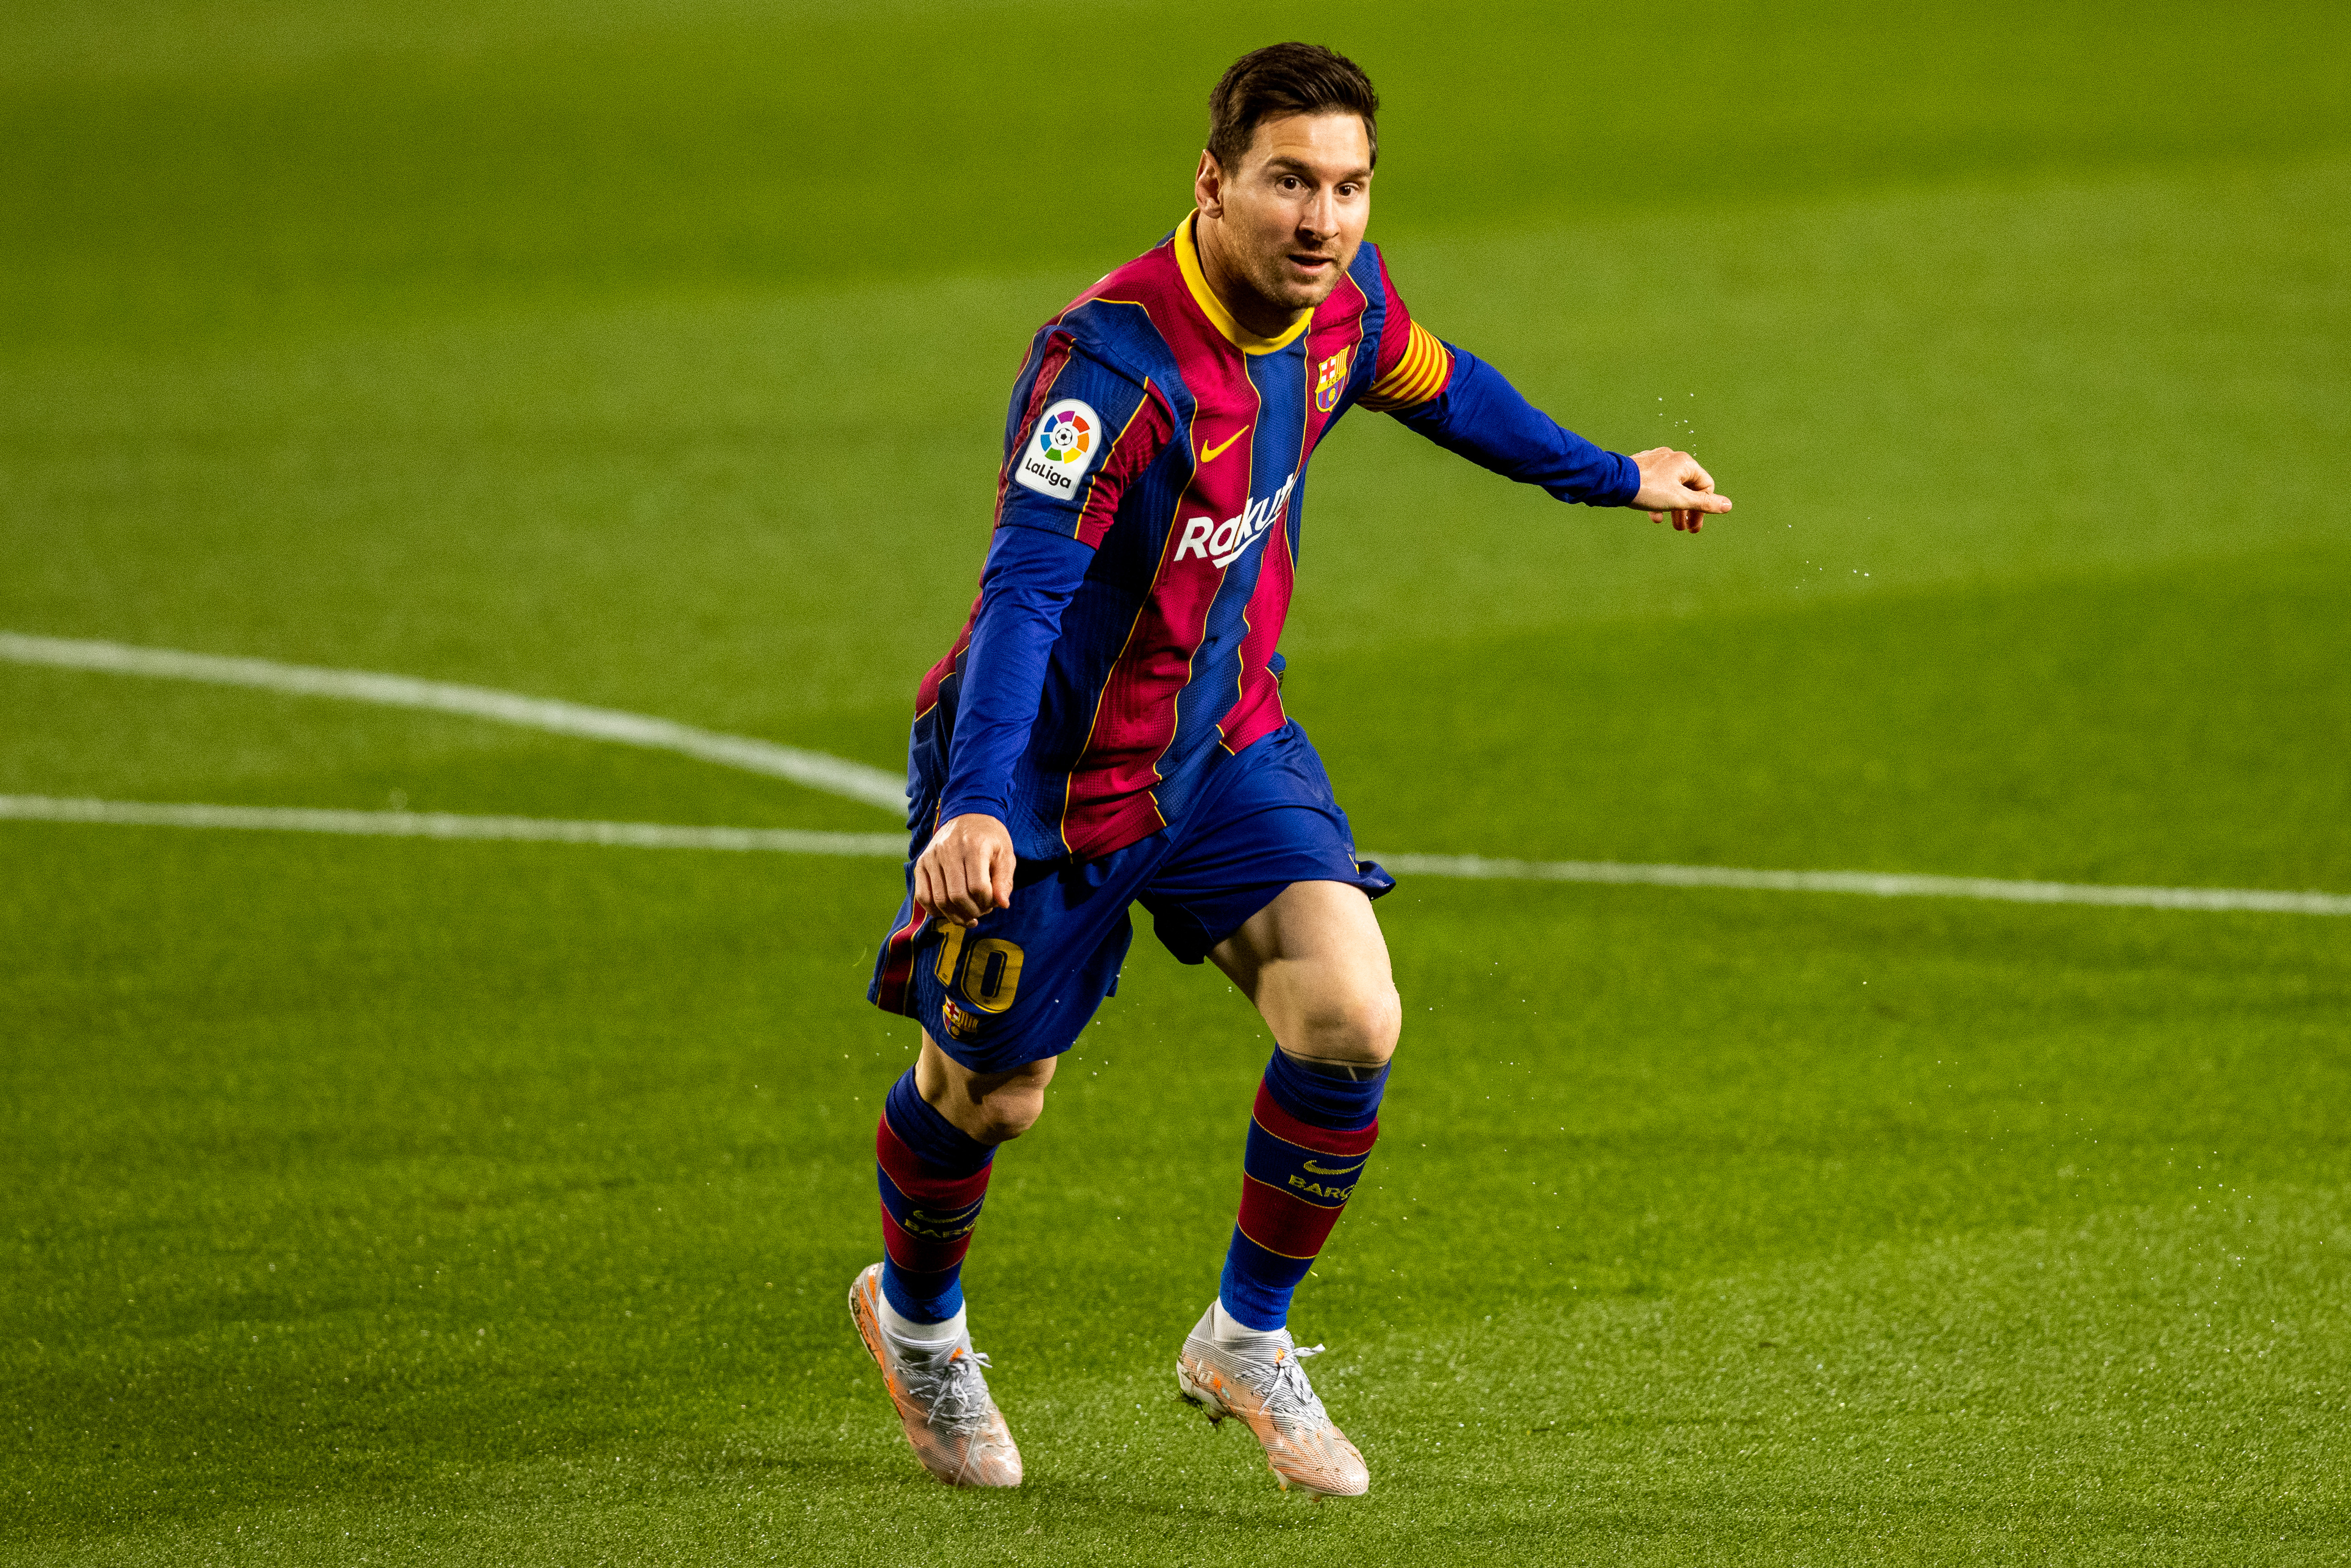
\includegraphics[width=\textwidth]{placeholder.jpg}
  \caption{Place Holder Image}
  \Description{Placeholder Image}
\label{fig:teaser}
\end{teaserfigure}



\begin{abstract}
  A clear and well-documented \LaTeX\ document is presented as an
  article formatted for publication by ACM in a conference proceedings
  or journal publication. Based on the ``acmart'' document class, this
  article presents and explains many of the common variations, as well
  as many of the formatting elements an author may use in the
  preparation of the documentation of their work.
\end{abstract}


\keywords{Do, Not, Use, This, Code, Put, the, Correct, Terms, for,
  Your, Paper}



%%
%% This command processes the author and affiliation and title
%% information and builds the first part of the formatted document.
\maketitle

\section{Introduction}
ACM's consolidated article template, introduced in 2017, provides a
consistent \LaTeX\ style for use across ACM publications, and
incorporates accessibility and metadata-extraction functionality
necessary for future Digital Library endeavors. Numerous ACM and
SIG-specific \LaTeX\ templates have been examined, and their unique
features incorporated into this single new template.

If you are new to publishing with ACM, this document is a valuable
guide to the process of preparing your work for publication. If you
have published with ACM before, this document provides insight and
instruction into more recent changes to the article template.

The ``\verb|acmart|'' document class can be used to prepare articles
for any ACM publication --- conference or journal, and for any stage
of publication, from review to final ``camera-ready'' copy, to the
author's own version, with {\itshape very} few changes to the source.


\section{Formation Change-Point Detection (FormCPD)}


\section{Role Change-Point Detection (RoleCPD)}
\subsection{Methodology}
The goal of RoleCPD \cite{Kim2022SoccerCPD} is to detect long-term tactical changes in player roles (e.g., a winger swapping sides with another winger permanently) while ignoring temporary switches (e.g., overlapping runs or covering defensive duties). This process operates within a single Formation Period $(T_i)$ identified in the previous step.

\subsection{Formal Representation}
We define the inputs and mathematiccal framework based on the SoccerCPD protocol:
\begin{itemize}
  \item \textbf{Input:} A sequence of "Temporary Role Permutations" $\{\pi_t\}_{t=1}^{|T_i|}$.
  \item \textbf{Role Permutation ($\pi_t$):} At every frame $t$, the Role Representation step assigns a role $X_p$ to every player $p$. Since roles are distinct, this assignement is a permutation of the initial canonical role: $$\beta_t (p) = \pi_t (X_p)$$ Where $\beta_t$ is the player-to-temporary-role mapping at time $t$.
\end{itemize}

\subsection{The Distance Metric}
To detect a change, we must quantify the difference between the team's configuration at time $t$ and time $t'$. Since the data consists of permutations (non-Euclidean), we cannot use standard Euclidean distance. We use the Hamming Distance normalized by the number of roles ($N = 10$ outfield players): $$d(\pi_t, \pi_{t'}) = \frac{1}{N} \sum_{p \in P} \mathbbm{1}_{\pi_t(X_p) \neq \pi_{t'}(X_p)}$$ This metric represents the "Switch Rate" or the proportion of players whose roles differ between two frames.

\subsection{Change-Point Detection Algorithm}
The paper utilizes Discrete g-segmentation, a graph-based change-point detection method effective for repeated observations in non-Euclidean space.
The procedure is as follows:
\begin{enumerate}
  \item \textbf{Preprocessing:} Calculate the Switch Rate relative to the dominant permutation. Exclude frames with a switch rate $> 0.7$ (likely temporary switches during set-pieces or abnormal situations).
  \item \textbf{Segmentation:} Apply the dectection algorithm recursively on the sequence of permutations using the Hamming distance.
  \item \textbf{Significance Test:} A change point $\tau$ is significant if:
    \begin{itemize}
      \item The p-value of the scan statistic is $< 0.01$.
      \item The segmentation duration is sufficient (robustness against noise).
      \item The most frequent permutations (Instructed Roles) in the segments before and after $\tau$ must be distinct.
    \end{itemize}
\end{enumerate}








%% The next two lines define the bibliography style to be used, and
%% the bibliography file.
\bibliographystyle{ACM-Reference-Format}
\bibliography{bib}

\end{document}
\endinput
%%
%% End of file `sample-sigconf.tex'.
